\chapter{RESULTS}
\label{ch:results}

Evaluating the BioBERT triage classifier requires a structured analysis of its foundational architecture, predictive performance under domain shift, and pathway implications. The initial phase establishes the computational baseline using the twelve-layer BioBERT architecture defined in Chapter~\ref{ch:method}. Primary reported metrics then come from \textbf{external} evaluation on the National Hospital Ambulatory Medical Care Survey (NHAMCS) 2018--22 and the Medical Information Mart for Intensive Care IV Emergency Department (MIMIC-IV-ED) open demo matching the v2.2 triage schema \citep{nhamcs201822,mimiciveddemo2023,mimicived2023}. Triagegeist is used for training and validation only. None of these sources is prospective live performance at \examplehospital{}.

\section{BioBERT model analysis}
\label{sec:biobert-analysis}

The first results question is not ``how accurate is the chatbot on a table?'' but ``what model is deployed, and does it work only after the right training?'' Before project-specific fine-tuning, the classifier rests on BioBERT-base \citep{lee2020biobert}: a twelve-layer bidirectional encoder with hidden dimension \(768\), twelve attention heads, project maximum sequence length \(M=128\) tokens (native BioBERT maximum is 512; Section~\ref{sec:tokenisation}), and a WordPiece vocabulary of approximately \(28{,}996\) tokens (Section~\ref{sec:encoder}). Stages~1 and~2 (Section~\ref{sec:training-pipeline}) supply biomedical language understanding and partial triage-oriented encoder features; they do \emph{not} produce the five-class acuity mapping required at intake. Stage~3 reinitialises the classification head and trains on the Triagegeist English corpus (Section~\ref{sec:data-provenance}). Class imbalance in the training corpus (Level~3 is the mode; Level~1 is the minority) motivates Stage~3 stratified oversampling documented in Section~\ref{sec:finetuned-analysis}.

Figure~\ref{fig:biobert-stack} summarises the three-stage training stack. Stage~1 applies masked language modelling on PubMed and PubMed Central text; Stage~2 transfers encoder weights from a prior two-class triage checkpoint with the old head discarded; Stage~3 is the comprehensive project fine-tuning that maps free-text complaints to five ESI-style acuity levels.

\begin{figure}[H]
\centering
\resizebox{0.92\textwidth}{!}{%
\begin{tikzpicture}[
  node distance=0.45cm and 0.35cm,
  stage/.style={draw=green!60!black, rounded corners, fill=green!8,
    minimum width=2.6cm, minimum height=0.85cm, align=center, font=\scriptsize},
  arrow/.style={->, >=latex, thick, draw=black!60}]
  \node[stage] (s1) {Stage 1\\BioBERT MLM\\PubMed + PMC};
  \node[stage, right=of s1] (s2) {Stage 2\\Encoder transfer\\2-class checkpoint};
  \node[stage, right=of s2] (s3) {Stage 3\\Project fine-tuning\\80k complaints, 5 classes};
  \node[stage, right=of s3, fill=triageYellow!25] (out) {Deployed\\triage model};
  \foreach \a/\b in {s1/s2, s2/s3, s3/out} \draw[arrow] (\a) -- (\b);
\end{tikzpicture}}
\caption{Three-stage BioBERT training stack (Stages~1--2 pre-date project fine-tuning; Stage~3 produces the deployed five-class head).}
\label{fig:biobert-stack}
\end{figure}

Read left to right, the diagram is a horizontal training pipeline: each box is one stage and the arrows show how parameters flow into the next. Stage~3 is the only stage that maps chief complaints to five acuity levels. The chatbot's urgency signal therefore depends on completing Stage~3; Stages~1--2 alone cannot route patients safely.

Naive bounds still motivate Stage~3: uniform random and an untrained head sit near 20\% five-class accuracy, and a majority-class rule (always Level~3) reaches about 36\% on Triagegeist with 0\% Red recall. Stages~1--2 alone therefore cannot route patients. Published headline performance is deferred to the external evaluation in Section~\ref{sec:finetuned-analysis} (Table~\ref{tab:external-metrics} and Figure~\ref{fig:external-metrics-compare}).

Figure~\ref{fig:biobert-model-specs} visualises the static dimensions of the deployed encoder.

\begin{figure}[H]
\centering
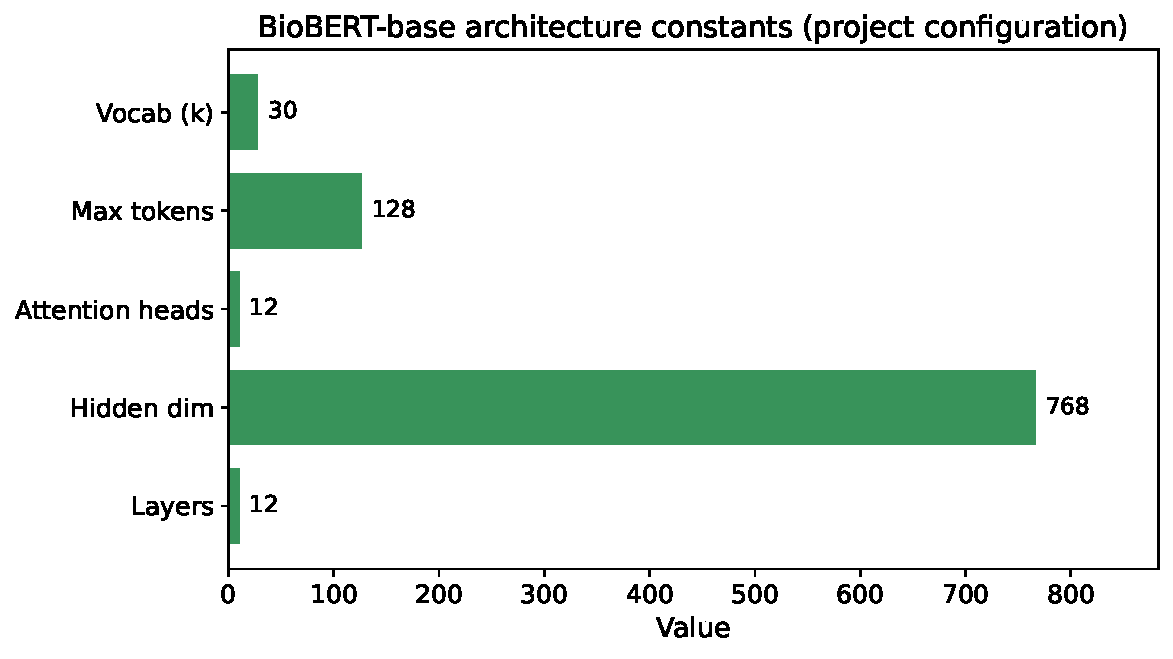
\includegraphics[width=0.88\textwidth]{figures/ch4/model_specs.pdf}
\caption{BioBERT-base architecture constants (project configuration; \(M=128\) is a deployment choice versus native length 512).}
\label{fig:biobert-model-specs}
\end{figure}

Figure~\ref{fig:biobert-model-specs} lists architecture parameter names on the vertical axis and their numeric values on the horizontal axis, drawn from the project \texttt{config.json} and the BioBERT-base specification \citep{lee2020biobert}. Layers (\(12\)), hidden dimension (\(768\)), and attention heads (\(12\)) are fixed by BioBERT-base. The maximum token length is deliberately constrained to \(M=128\) (versus the native BioBERT maximum of \(512\)) to keep intake inference sub-second; the vocabulary is approximately \(30{,}000\) tokens.

\section{Fine-tuned model analysis}
\label{sec:finetuned-analysis}

Having established the BioBERT configuration and the necessity of Stage~3 fine-tuning, the remainder of this chapter reports \textbf{external} predictive metrics, colour accuracy via \(f_{\mathrm{SATS}}\), under/over-triage, and pathway implications.

\subsection{Evaluation protocol}
\label{sec:eval-protocol}

Primary reported metrics are from external evaluation on MIMIC-IV-ED and NHAMCS. Triagegeist is used for training/validation only. None of these sources is prospective live performance at \examplehospital{}.

\begin{enumerate}
\item \textbf{Train / validation (Triagegeist).} Stratified 90/10 split (seed~42) for Stage~3 fine-tuning and checkpoint selection. No Triagegeist holdout accuracy is reported as a Results headline.
\item \textbf{External A: MIMIC-IV-ED.} Text-only on \texttt{chiefcomplaint} \(\rightarrow\) predict acuity; gold = \texttt{acuity} \(\in\{1,\ldots,5\}\). Full MIMIC-IV-ED v2.2 is credentialed on PhysioNet \citep{mimicived2023}; this project evaluates the open demo matching the same triage schema \citep{mimiciveddemo2023} (\(N=207\) after filters) until a full extract is available.
\item \textbf{External B: NHAMCS 2018--22.} Text-only on \texttt{chief\_complaint\_text} \(\rightarrow\) predict acuity; gold = \texttt{target\_triage\_acuity} \citep{nhamcs201822}. After filters, \(N=58{,}124\) rows remain; metrics below use a stratified subsample of \(N=12{,}000\) (seed~42) for compute, with full-set class support reported in Table~\ref{tab:external-support}.
\end{enumerate}

\textbf{Pre-processing (both external sets).} Drop empty, NaN, or whitespace-only complaints; keep acuity in \(\{1,\ldots,5\}\); do \emph{not} expand nursing abbreviations (e.g.\ CP, SOB); tokenise with BioBERT WordPiece and truncate/pad to project length \(M=128\).

Two checkpoints are compared:

\begin{enumerate}
\item \textbf{Baseline fine-tuned BioBERT} (project default): end-to-end fine-tuning without minority rebalancing beyond the natural train distribution.
\item \textbf{Stratified-oversampling variant:} text augmentation plus random minority oversampling on the Triagegeist training split, then end-to-end fine-tuning (Section~\ref{sec:oversampling-choice}).
\end{enumerate}

Metrics: five-class accuracy and macro-F1; 4-colour accuracy after \(f_{\mathrm{SATS}}\); under-triage (predicted less urgent than true); over-triage (more urgent); critical under-triage (true Red\(\rightarrow\)non-Red; true Orange\(\rightarrow\)Yellow/Green); latency.

\subsection{Acuity distribution on test sets}
\label{sec:external-support}

Table~\ref{tab:external-support} reports gold acuity counts by level after the shared pre-processing in Section~\ref{sec:eval-protocol}. The NHAMCS counts come from the 2018--22 US emergency-department survey text field \texttt{chief\_complaint\_text} with gold labels \texttt{target\_triage\_acuity} \citep{nhamcs201822}: \(N=58{,}124\) rows after filters, with the stratified evaluation subsample (\(N=12{,}000\)) used for published metrics. The MIMIC counts come from the open MIMIC-IV-ED demo on PhysioNet (Boston ED phrasing), mapping \texttt{chiefcomplaint} to gold \texttt{acuity} \citep{mimiciveddemo2023} (\(N=207\) after filters). Real emergency departments are imbalanced: NHAMCS is dominated by Levels~3--4, and Level~1 is scarce (846 of 58{,}124; 1.5\%). MIMIC demo counts are small, especially Levels~4--5, so rare-class metrics there are interpreted cautiously.

\begin{table}[H]
\centering
\small
\begin{tabular}{|l|r|r|r|r|r|r|}
\hline
\textbf{Set} & \(N_1\) & \(N_2\) & \(N_3\) & \(N_4\) & \(N_5\) & \textbf{Total} \\
\hline
NHAMCS (full retained) & 846 & 8{,}597 & 29{,}568 & 16{,}715 & 2{,}398 & 58{,}124 \\
NHAMCS (eval subsample) & 175 & 1{,}775 & 6{,}104 & 3{,}451 & 495 & 12{,}000 \\
MIMIC-IV-ED demo & 18 & 97 & 90 & 2 & 0 & 207 \\
\hline
\end{tabular}
\caption{Gold acuity counts by level on the NHAMCS and MIMIC-IV-ED demo test sets after pre-processing.}
\label{tab:external-support}
\end{table}

\subsection{Why prior in-distribution accuracy looked inflated}
\label{sec:high-accuracy}

A Triagegeist duplicate analysis finds only 4{,}949 unique normalised complaint strings among 80{,}000 training rows (duplicate rate \(\approx 93.8\%\); 4{,}184 templates appear at least five times). High template reuse helps explain why earlier in-distribution holdout figures near 99.9\% looked unrealistically strong: they largely measure agreement on repeated synthetic phrasing, not generalisation. Those figures are therefore retired from the Results headline in favour of MIMIC/NHAMCS metrics below.

\subsection{Stratified oversampling for class imbalance}
\label{sec:oversampling-choice}

Stage~3 training on Triagegeist is class-imbalanced: Level~3 (Urgent) is the mode, while Level~1 (Resuscitation / Red) is the minority. Rebalancing the training split can raise Red recall, but often at a cost to precision and overall accuracy. Two natural ways to reduce that imbalance were available for this project.

\textbf{A: Classical embedding SMOTE.} Raw chief-complaint strings are discrete, so SMOTE cannot interpolate between token sequences directly \citep{chawla2002smote}. One workable route is to freeze (or otherwise detach) BioBERT, extract fixed feature vectors such as \(h_{[\mathrm{CLS}]}\in\mathbb{R}^{768}\), apply SMOTE in that continuous space to synthesise minority examples, and train a \emph{separate} linear classification head on the resulting embedding set. Gradients never update the text encoder during that second stage.

\textbf{B: Stratified oversampling (chosen).} Keep the end-to-end Stage~3 pipeline of Chapter~\ref{ch:method}: WordPiece tokenisation, BioBERT encoder, and Softmax head trained jointly. On the Triagegeist \emph{training} split only, apply text augmentation to minority urgent classes, then random minority oversampling toward configured target counts, and continue full encoder-plus-head updates. The training configuration sets \texttt{USE\_EMBEDDING\_SMOTE=False}, so embedding-space SMOTE is not part of the published second checkpoint.

This project adopts \textbf{B} for the published imbalance-mitigated checkpoint and does \emph{not} report a classical embedding-SMOTE model as the official second result.

The choice follows from the training objective. End-to-end Stage~3 is meant to adapt WordPiece and attention features to short chief-complaint language; that requires backpropagation into BioBERT. SMOTE-generated points in embedding space cannot be pushed back through the text encoder unless BioBERT is frozen, which would abandon that adaptation goal and replace it with a shallow head on static features. Stratified oversampling instead keeps real or lightly paraphrased complaint text inside the same tokenizer \(\rightarrow\) encoder \(\rightarrow\) Softmax path already specified in Chapter~\ref{ch:method}. Calling B ``SMOTE'' would therefore be inaccurate for the panel: Chawla-style SMOTE \citep{chawla2002smote} describes A, which was considered but not used for the published checkpoint.

The NHAMCS and MIMIC comparisons below therefore contrast the baseline Stage~3 model with this stratified-oversampling checkpoint, not with an embedding-SMOTE head.

\subsection{NHAMCS external results}
\label{sec:nhamcs-results}

On the stratified NHAMCS subsample (\(N=12{,}000\)), baseline BioBERT reaches 47.60\% five-class accuracy, 0.288 macro-F1, and 49.95\% colour accuracy after \(f_{\mathrm{SATS}}\) (Table~\ref{tab:external-metrics}). Under-triage is 28.39\% and over-triage 24.01\%. Level~1 recall is only 8.00\% (support 175) despite 82.35\% Level~1 precision: most true Red cases are predicted as Orange or Yellow (Figure~\ref{fig:confusion-nhamcs-baseline}), which is the primary safety concern under domain shift \citep{Berkowitz2019}.

\begin{table}[H]
\centering
\small
\begin{tabular}{|l|r|r|r|r|}
\hline
\textbf{Metric} & \textbf{NHAMCS base.} & \textbf{NHAMCS overs.} & \textbf{MIMIC base.} & \textbf{MIMIC overs.} \\
\hline
\(N\) & 12{,}000 & 12{,}000 & 207 & 207 \\
Accuracy & 0.4760 & 0.3045 & 0.3043 & 0.2126 \\
Macro-F1 & 0.2882 & 0.2146 & 0.1748 & 0.1781 \\
Colour accuracy & 0.4995 & 0.3422 & 0.3043 & 0.2126 \\
Under-triage & 0.2839 & 0.3903 & 0.6377 & 0.6087 \\
Over-triage & 0.2401 & 0.3052 & 0.0580 & 0.1787 \\
Recall L1 (Red) & 0.0800 & 0.2171 & 0.1111 & 0.5000 \\
Precision L1 & 0.8235 & 0.0597 & 0.4000 & 0.2647 \\
Latency p50 (ms) & 94.00 & 96.18 & n/a & n/a \\
\hline
\end{tabular}
\caption{External classification, colour, under/over-triage, and latency metrics. MIMIC columns use the open demo (\(N=207\)). MIMIC latency is reported as n/a: published timing uses the NHAMCS evaluation run (Section~\ref{sec:latency}).}
\label{tab:external-metrics}
\end{table}

\begin{figure}[H]
\centering
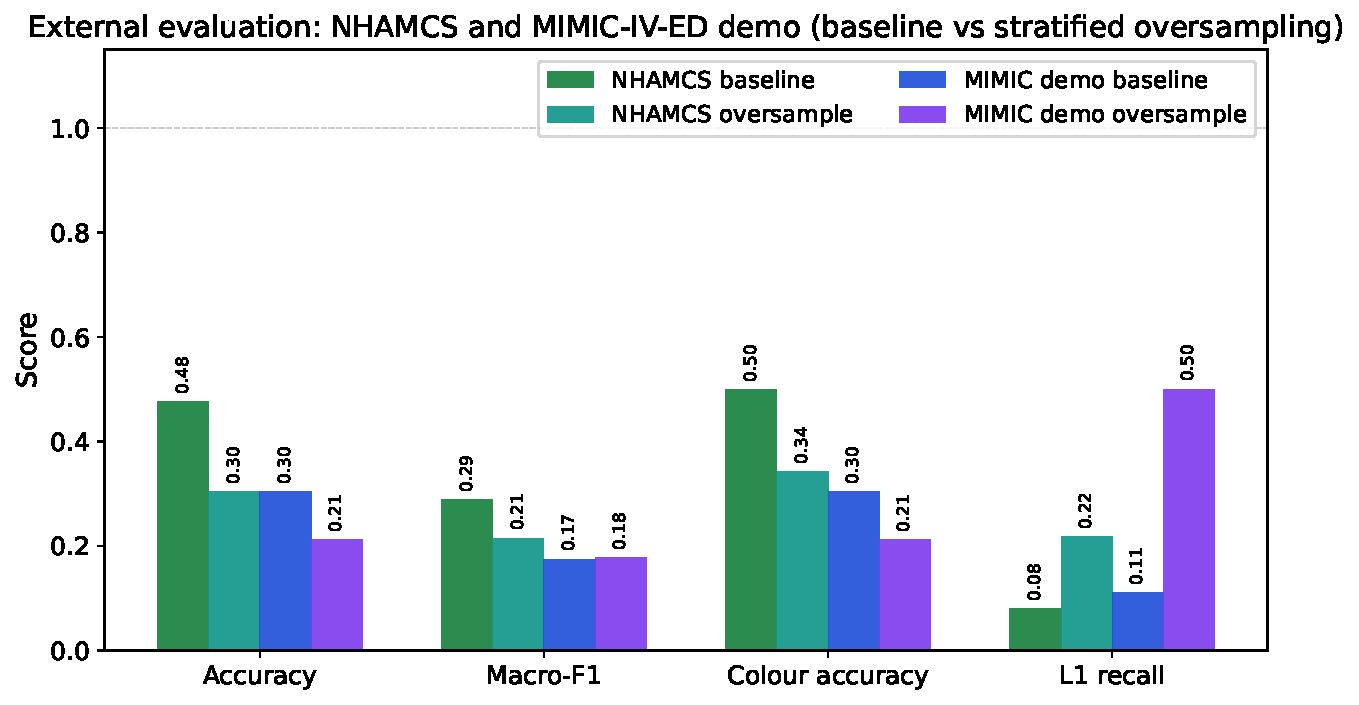
\includegraphics[width=0.92\textwidth]{figures/ch4/external_metrics_compare.pdf}
\caption{External headline metrics on NHAMCS (\(N=12{,}000\) stratified subsample) and MIMIC-IV-ED demo (\(N=207\)): baseline versus stratified oversampling.}
\label{fig:external-metrics-compare}
\end{figure}

Figure~\ref{fig:external-metrics-compare} plots the same accuracy, macro-F1, colour accuracy, and Level~1 recall values as Table~\ref{tab:external-metrics}, so the baseline--oversample contrast is readable before the confusion matrices below.

\begin{figure}[H]
\centering
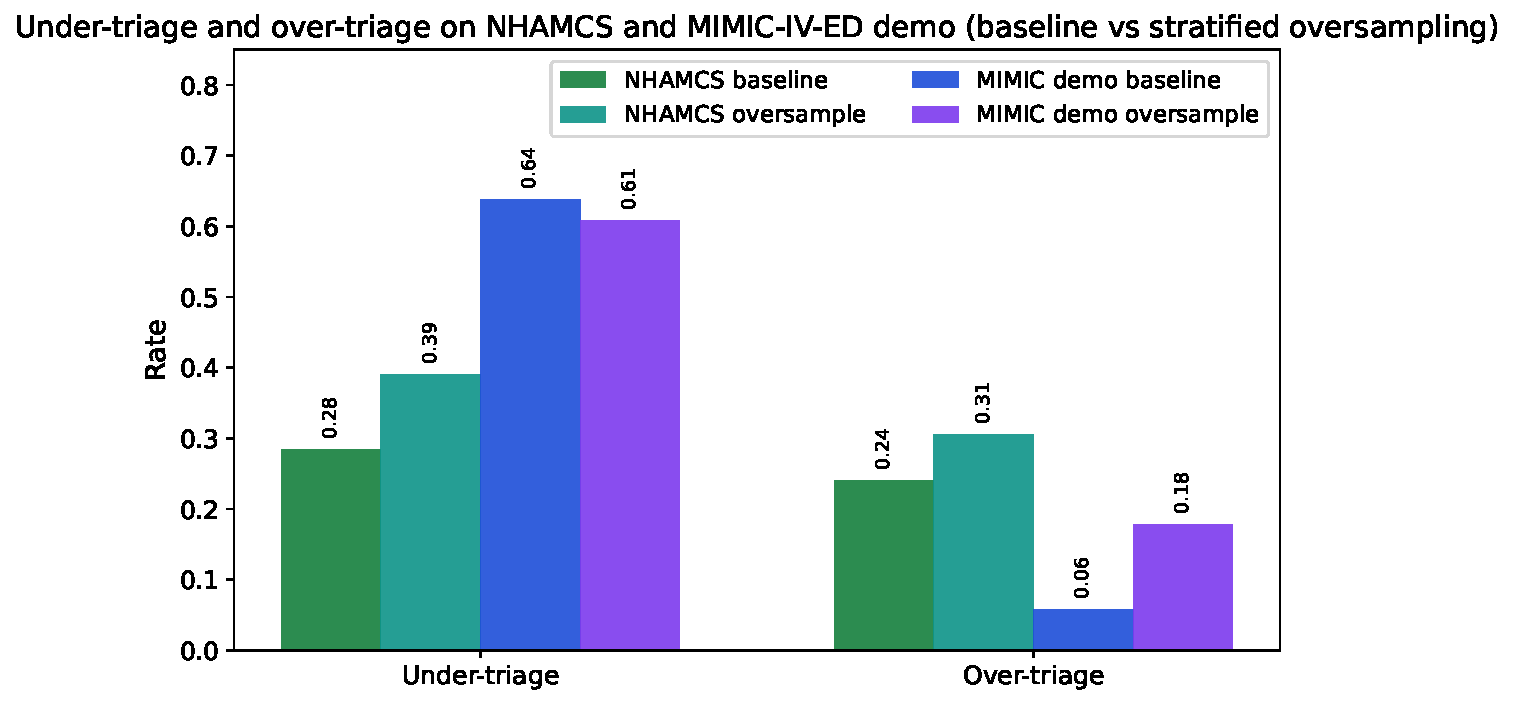
\includegraphics[width=0.92\textwidth]{figures/ch4/external_under_over_triage.pdf}
\caption{Under-triage and over-triage rates on NHAMCS (\(N=12{,}000\) stratified subsample) and MIMIC-IV-ED demo (\(N=207\)): baseline versus stratified oversampling.}
\label{fig:external-under-over-triage}
\end{figure}

Under-triage (predicted less urgent than gold) is the safety failure mode: urgent language is routed too late. Over-triage (predicted more urgent than gold) is false escalation that loads acute streams and staff. Figure~\ref{fig:external-under-over-triage} shows that on NHAMCS, stratified oversampling raises \emph{both} under-triage (28.39\% to 39.03\%) and over-triage (24.01\% to 30.52\%) even while Level~1 recall rises (Figure~\ref{fig:external-metrics-compare}, Table~\ref{tab:external-metrics}), so sensitivity gains are not a free improvement in directional error. On the MIMIC demo, baseline under-triage is already high (63.77\%); oversampling mainly increases over-triage (5.80\% to 17.87\%). These patterns reinforce mandatory nurse override under domain shift \citep{Berkowitz2019}.

\begin{figure}[H]
\centering
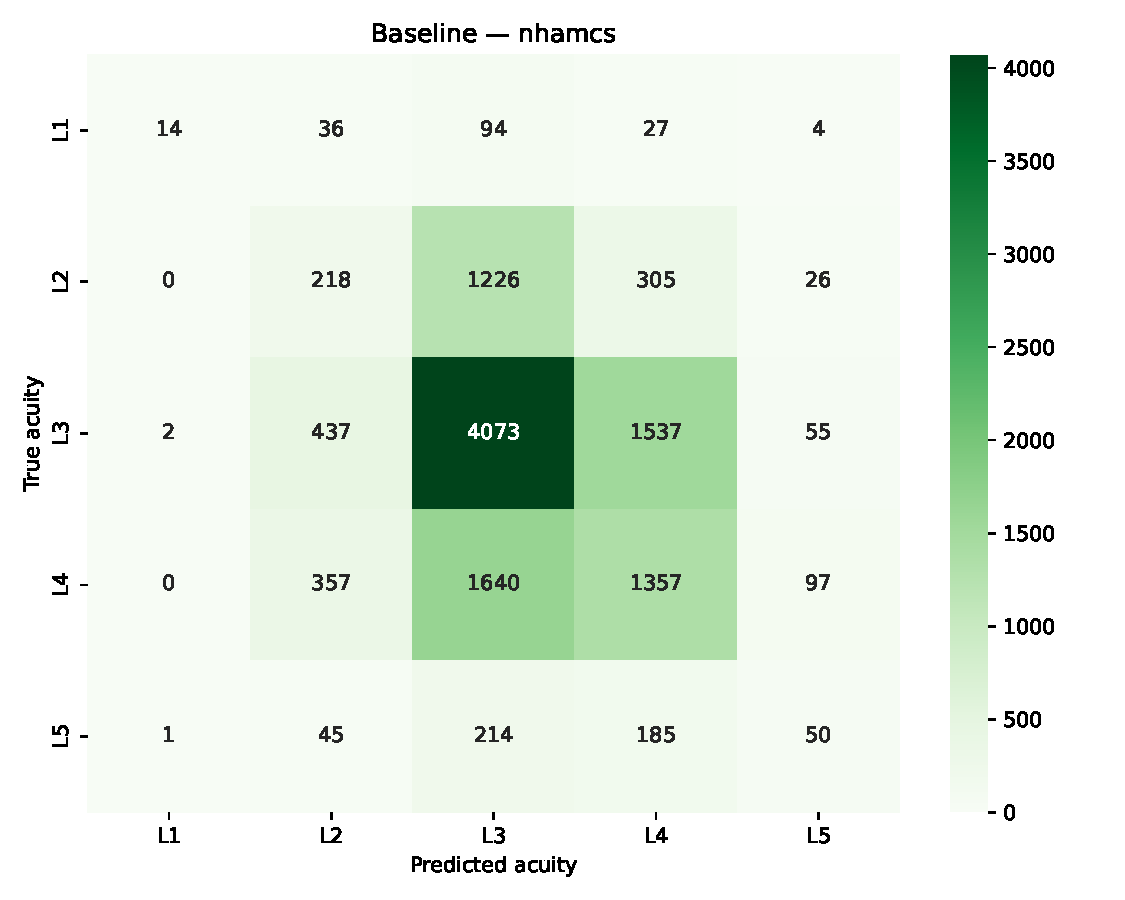
\includegraphics[width=0.82\textwidth]{figures/ch4/nhamcs_baseline_confusion.pdf}
\caption{Baseline BioBERT confusion matrix on NHAMCS stratified subsample (\(N=12{,}000\)). Rows = true acuity; columns = prediction. Dark diagonal cells are correct predictions; off-diagonal mass is triage error.}
\label{fig:confusion-nhamcs-baseline}
\end{figure}

The NHAMCS baseline matrix shows substantial off-diagonal mass. Of 175 true Level~1 cases, only 14 are recovered; 36 are predicted Level~2 (Orange) and 94 Level~3 (Yellow). Under-triage of critical presentations therefore dominates residual error on this US survey set.

\begin{figure}[H]
\centering
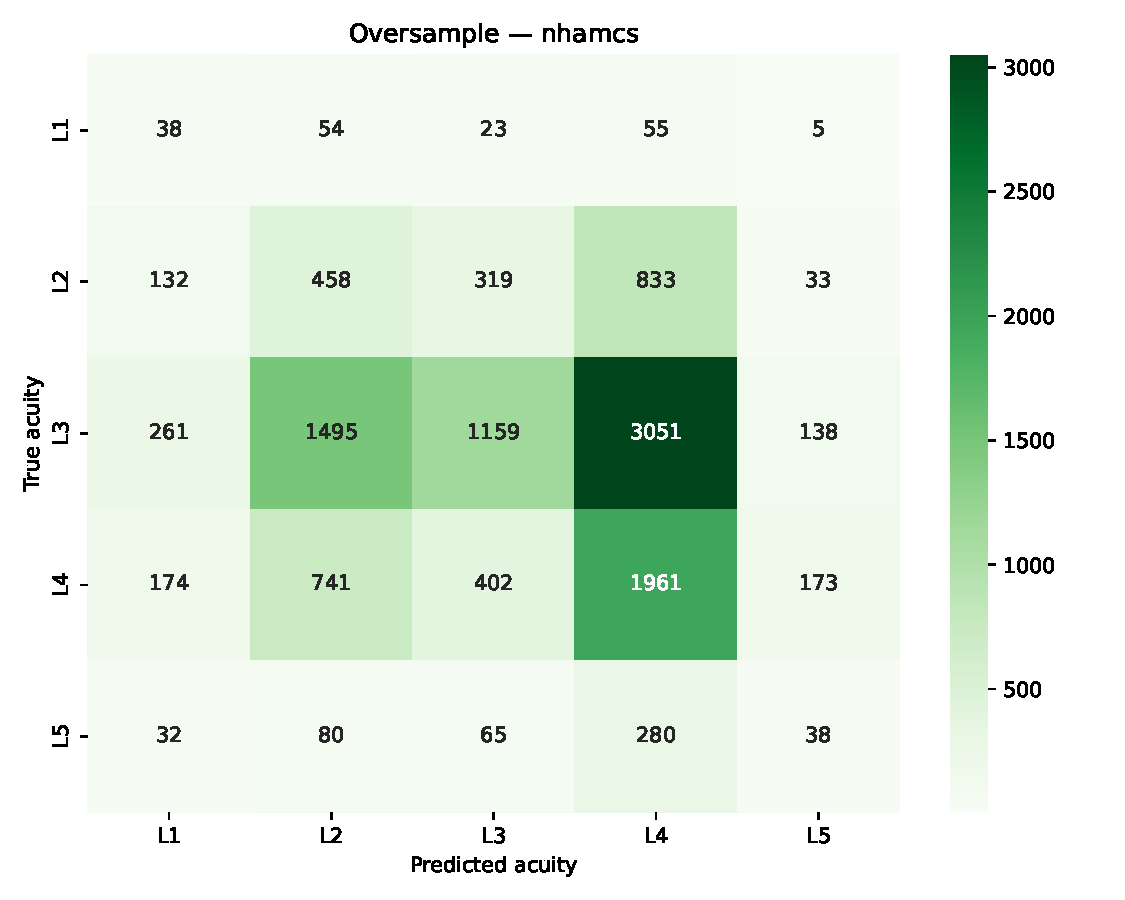
\includegraphics[width=0.82\textwidth]{figures/ch4/nhamcs_oversample_confusion.pdf}
\caption{Stratified-oversampling BioBERT confusion matrix on the same NHAMCS subsample. Dark diagonal cells are correct predictions; off-diagonal mass is triage error.}
\label{fig:confusion-nhamcs-oversample}
\end{figure}

Stratified oversampling raises NHAMCS Level~1 recall from 8.00\% to 21.71\% but lowers overall accuracy to 30.45\% and Level~1 precision to 5.97\%: more false urgent alerts accompany the sensitivity gain. As visually demonstrated by the drop in the Accuracy bars in Figure~\ref{fig:external-metrics-compare}, stratified oversampling trades overall exact-match accuracy to raise Level~1 recall (Table~\ref{tab:external-metrics}). The baseline checkpoint remains the project default unless stakeholders explicitly prioritise Red sensitivity over precision \citep{Berkowitz2019}.

\subsection{MIMIC-IV-ED demo results}

On the open MIMIC-IV-ED demo (\(N=207\)), baseline accuracy is 30.43\% with colour accuracy 30.43\% and high under-triage (63.77\%). As shown in the baseline matrix (Figure~\ref{fig:confusion-mimic-baseline}), the model correctly recovers only 2 of 18 true Level~1 cases. With stratified oversampling (Figure~\ref{fig:confusion-mimic-oversample}), this increases to 9 of 18 cases (50.00\% recall), though the matrix shows a corresponding spread of false positives across Levels~2 and~3, and overall accuracy falls to 21.26\%. These demo figures validate the evaluation pipeline on real Boston ED phrasing but are not substitutes for a full credentialed MIMIC-IV-ED v2.2 extract \citep{mimicived2023}.

\begin{figure}[H]
\centering
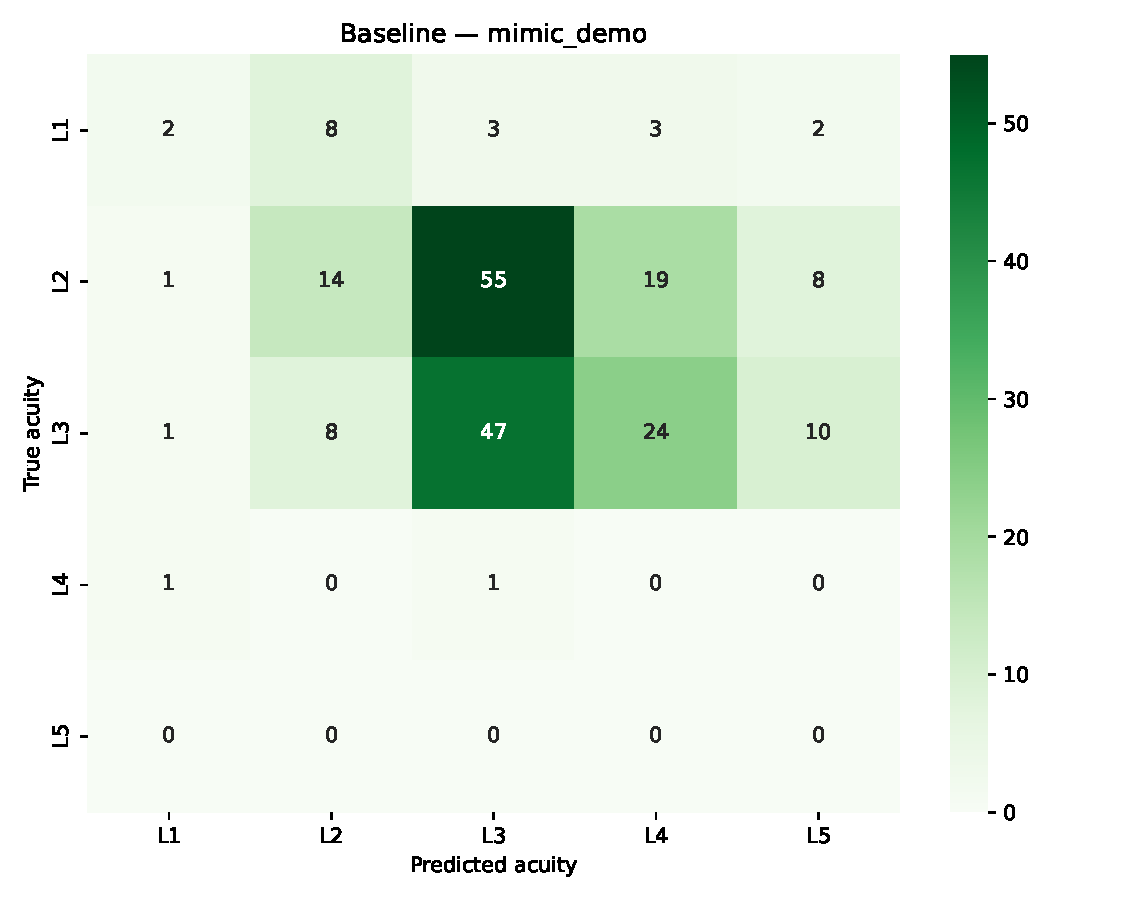
\includegraphics[width=0.82\textwidth]{figures/ch4/mimic_demo_baseline_confusion.pdf}
\caption{Baseline BioBERT confusion matrix on MIMIC-IV-ED demo (\(N=207\)). Rows = true acuity; columns = prediction. Dark diagonal cells are correct predictions; off-diagonal mass is triage error.}
\label{fig:confusion-mimic-baseline}
\end{figure}

\begin{figure}[H]
\centering
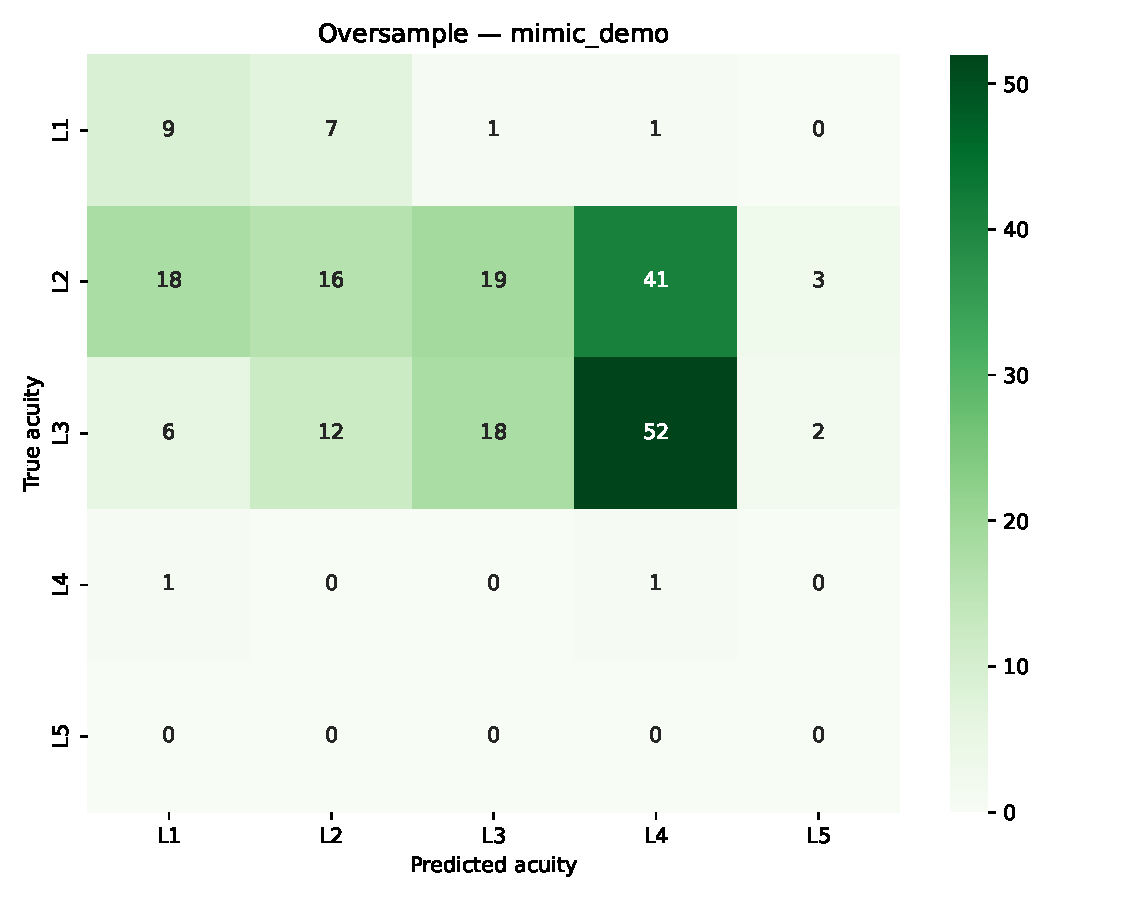
\includegraphics[width=0.82\textwidth]{figures/ch4/mimic_demo_oversample_confusion.pdf}
\caption{Stratified-oversampling BioBERT confusion matrix on MIMIC-IV-ED demo. Dark diagonal cells are correct predictions; off-diagonal mass is triage error.}
\label{fig:confusion-mimic-oversample}
\end{figure}

\subsection{Colour accuracy and under/over-triage}

Mapping levels through \(f_{\mathrm{SATS}}\) (Table~\ref{tab:fsats-esi}) yields 4-colour accuracy at or above five-class accuracy when Levels~4 and~5 both map to Green. On NHAMCS baseline, colour accuracy (49.95\%) slightly exceeds five-class accuracy (47.60\%). Critical under-triage of true Red to non-Red remains high (92.00\% baseline NHAMCS; 78.29\% oversampled), reinforcing mandatory nurse override for urgent language \citep{Berkowitz2019}.

\subsection{Inference latency}
\label{sec:latency}

Real-time intake requires sub-second response \citep{stewart2023nlp}. Latency in Table~\ref{tab:external-metrics} is a property of the BioBERT forward pass at project length \(M=128\) on the evaluation hardware, not a dataset-specific accuracy score. The published timing benchmark is therefore the NHAMCS stratified subsample (\(N=12{,}000\)), which is large enough for stable median and tail estimates: baseline median latency \(\approx 94\)\,ms (p95 \(\approx 124\)\,ms); the stratified-oversampling checkpoint is similar (p50 \(\approx 96\)\,ms). Both respond in well under one second, supporting chatbot intake before nurse vitals are recorded.

MIMIC-IV-ED demo columns in the same table show n/a for latency by design. That demo (\(N=207\)) is used for external accuracy, colour accuracy, and under/over-triage only. A second latency estimate on so few batches would not change the operational sub-second claim and would overstate the precision of a short timing sample. The same checkpoints and the same \(M=128\) truncation are used on both externals, so the NHAMCS p50 already represents chatbot response time at intake.

\begin{remark}
External metrics are substantially lower than earlier Triagegeist in-distribution figures, as expected under geographic and demographic domain shift (Chapter~\ref{ch:conclusion}). Text still carries a partial acuity signal, but the chatbot must remain nurse-overridable.
\end{remark}

\section{Pathway routing at \examplehospital{}}
\label{sec:pathway-results}

The complete five-scenario pathway map (gate reject plus Red, Orange, Yellow, Green) is specified in Tables~\ref{tab:pathway-scenarios} and~\ref{tab:pathway-examples} and illustrated in Figure~\ref{fig:pathway-map}. Each scenario assigns primary clinical departments, support actions across Nursing, Pharmacy, Health Information, Hospital Information Technology, Administration, and Accounts, and an escalation rule \citep{satsmanual,Rominski2014}.

\subsection{Nurse triage vs chatbot response}
\label{sec:nurse-vs-chatbot}

Table~\ref{tab:nurse-vs-chatbot} contrasts manual nurse triage with the hospital chatbot on dimensions relevant to intake at \examplehospital{}. Nurse-side timings are drawn from published LMIC triage literature; chatbot timings are measured on the external evaluation hardware.

\begin{table}[H]
\centering
\small
\begin{tabular}{|p{3.2cm}|p{5.2cm}|p{5.2cm}|}
\hline
\textbf{Dimension} & \textbf{Manual nurse triage} & \textbf{Hospital chatbot (this project)} \\
\hline
Time to first acuity signal &
Queue-dependent; LMIC intake often delayed minutes to hours before nurse contact \citep{kathsats,Mitchell2023,Nurchis2025} &
Approximately 94--100\,ms inference on evaluation hardware (Table~\ref{tab:external-metrics}) \\
Inputs used &
Chief complaint + vitals + TEWS + clinical judgment \citep{satsmanual} &
Text-only chief complaint; TEWS applied separately by nurse (Section~\ref{sec:tews}) \\
Output &
SATS colour + bedside assessment &
SATS colour + pathway card + confidence score \\
Validation basis &
Live clinical decision at triage desk &
External offline agreement on MIMIC/NHAMCS text (Section~\ref{sec:nhamcs-results}) \\
Role at \examplehospital{} &
Authoritative triage &
Triage assist at arrival; nurse override mandatory for low confidence and all vitals \citep{stewart2023nlp} \\
\hline
\end{tabular}
\caption{Manual nurse triage versus chatbot assist at intake.}
\label{tab:nurse-vs-chatbot}
\end{table}

Once the chatbot assigns a colour in approximately 100\,ms, pathway timer rules take effect: Orange cases require clinician contact within ten minutes, Yellow within 60 minutes, and Green within four hours (Section~\ref{sec:pathways}, Table~\ref{tab:pathway-scenarios}) \citep{satsmanual,Sundstrom2014}. The chatbot does not replace nurse assessment; it provides an immediate acuity signal so that queue time before \emph{any} routing decision is reduced relative to waiting for a free triage nurse \citep{Mitchell2023,Nurchis2025}.

\textbf{Gate rejection.} Non-clinical input receives no colour; Nursing re-prompts for a chief complaint. This prevents meaningless acuity scores and keeps acute queues free of idle interactions.

\textbf{Red.} Life-threatening text (e.g.\ crushing chest pain with dyspnoea) routes immediately to Surgery and Internal Medicine with Code Red alerts via HIT. Administration bypasses routine registration so resuscitation is not delayed \citep{satsmanual}.

\textbf{Orange.} Very urgent complaints (e.g.\ severe abdominal pain in pregnancy) activate Internal Medicine, Surgery, or Obstetrics and Gynaecology within ten minutes, with stat Diagnostics and a head-nurse escalation if unclaimed.

\textbf{Yellow.} For the running illustrative complaint (\runningcomplaint{}), the model assigns level 3 at approximately 72\% confidence. The pathway card routes to the Outpatient urgent stream and parallel Diagnostics under the adult ASTS default; Pediatrics is used only when the complaint contains explicit child markers. Nursing sets a 60-minute reassessment timer.

\textbf{Green.} Routine presentations (e.g.\ dental pain without fever) divert to Outpatient, Dental, Eye, or Public and Preventive Health within four hours, reducing congestion in acute waiting areas \citep{Yilmaz2021,Sundstrom2014}.

Classification output (colour + confidence + department list) is the machine-readable input to this routing layer. External evaluation (Section~\ref{sec:nhamcs-results}) bounds offline reliability under domain shift; live intake at \examplehospital{} still requires nurse override.

\section{Anticipated impact on healthcare delivery}
\label{sec:impact}

The following analysis interprets how the chatbot can support faster, clearer hospital flow at \examplehospital{}, drawing on external metrics where available and on published triage literature elsewhere. No prospective waiting-time trial has yet been conducted at \examplehospital{} \citep{Mitchell2023}.

\subsection{Functional chatbot and workflow improvement}

We anticipate a functional chatbot that suggests urgency from a single chief complaint and supports hospital workflow by assigning SATS colour and department direction at intake \citep{stewart2023nlp,Mitchell2023}. External NHAMCS evaluation reports 47.60\% five-class accuracy and 49.95\% colour accuracy for the baseline checkpoint (Section~\ref{sec:nhamcs-results}), indicating that text carries a partial acuity signal under domain shift rather than near-perfect agreement. Median inference latency of approximately 94--100\,ms on evaluation hardware supports rapid digital response at arrival (Table~\ref{tab:nurse-vs-chatbot}).

Figure~\ref{fig:anticipated-workflow} compares time-to-first-acuity-signal: traditional intake (top) waits for a nurse; chatbot-assisted intake (bottom) classifies text immediately and runs nurse vitals in parallel.

\begin{figure}[H]
\centering
\resizebox{\textwidth}{!}{%
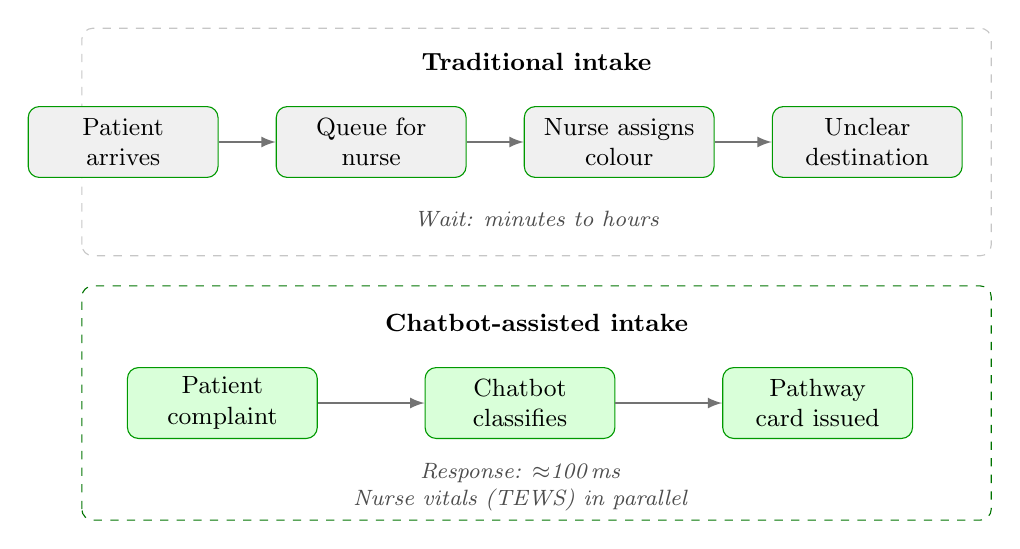
\begin{tikzpicture}[
  x=1.05cm, y=0.85cm,
  title/.style={font=\small\bfseries, anchor=center},
  box/.style={draw=green!60!black, rectangle, fill=green!10, text width=2.2cm, align=center,
    minimum height=0.9cm, rounded corners, font=\small, inner sep=3pt},
  old/.style={box, fill=gray!12},
  new/.style={box, fill=green!15},
  arrow/.style={->, >=latex, thick, draw=black!55},
  foot/.style={font=\footnotesize\itshape, text=black!70, align=center}]
  % Top panel: Traditional
  \node[title] at (5.0, 7.2) {Traditional intake};
  \draw[dashed, rounded corners, draw=gray!45] (-0.5, 4.3) rectangle (10.5, 7.7);
  \node[old] (q) at (0, 6.0) {Patient\\arrives};
  \node[old] (wait) at (3.0, 6.0) {Queue for\\nurse};
  \node[old] (nurse) at (6.0, 6.0) {Nurse assigns\\colour};
  \node[old] (unclear) at (9.0, 6.0) {Unclear\\destination};
  \draw[arrow] (q) -- (wait);
  \draw[arrow] (wait) -- (nurse);
  \draw[arrow] (nurse) -- (unclear);
  \node[foot] at (5.0, 4.85) {Wait: minutes to hours};
  % Bottom panel: Chatbot-assisted
  \node[title] at (5.0, 3.3) {Chatbot-assisted intake};
  \draw[dashed, rounded corners, draw=green!45!black] (-0.5, 0.35) rectangle (10.5, 3.85);
  \node[new] (c) at (1.2, 2.1) {Patient\\complaint};
  \node[new] (bot) at (4.8, 2.1) {Chatbot\\classifies};
  \node[new] (card) at (8.4, 2.1) {Pathway\\card issued};
  \draw[arrow] (c) -- (bot);
  \draw[arrow] (bot) -- (card);
  \node[foot] at (4.8, 1.05) {Response: \(\approx\)100\,ms};
  \node[foot] at (4.8, 0.65) {Nurse vitals (TEWS) in parallel};
\end{tikzpicture}}
\caption{Stacked intake comparison at \examplehospital{}. \textbf{Top:} patient queues minutes to hours before a nurse assigns colour. \textbf{Bottom:} chatbot classifies the complaint in \(\approx\)100\,ms and issues a pathway card; nurse vitals continue in parallel. Colour routing (Red/Orange vs Green) is detailed in Section~\ref{sec:pathway-results}.}
\label{fig:anticipated-workflow}
\end{figure}

The stacked workflow diagram has two panels read left to right. The top panel is traditional intake (arrive \(\rightarrow\) queue \(\rightarrow\) nurse assigns colour \(\rightarrow\) unclear destination); the bottom panel is chatbot-assisted intake (complaint \(\rightarrow\) chatbot classifies \(\rightarrow\) pathway card issued). Pathway design comes from Chapter~\ref{ch:method}, chatbot latency from the external evaluation in Section~\ref{sec:latency}, and traditional wait times from LMIC triage literature \citep{kathsats,Mitchell2023}. The top footnote reads ``Wait: minutes to hours''; the bottom footnotes read ``Response: \(\approx\)100\,ms'' and ``Nurse vitals (TEWS) in parallel''. Red/Orange fast-track and Green digital queue are developed in Section~\ref{sec:pathway-results}. The figure therefore contrasts slow nurse-queue intake with immediate chatbot classification while making clear that nurse assessment is not replaced \citep{satsmanual,stewart2023nlp}.

\subsection{Reduced initial triage wait times}

Published triage literature suggests wait times for initial triage may decrease when patients interact with the bot immediately rather than queue for a nurse \citep{Mitchell2023,Nurchis2025}. External evaluation shows the model can assign colour and pathway in approximately 100\,ms once valid clinical text is submitted (Table~\ref{tab:nurse-vs-chatbot}). Non-urgent (Green) cases can be digitally queued for later consultation while urgent cases are fast-tracked through Red and Orange escalation rules (Table~\ref{tab:pathway-scenarios}), potentially reducing overall waiting duration \citep{Sundstrom2014,Yilmaz2021}. Parallel diagnostics orders flagged on Yellow and Green pathway cards may further shorten total time to definitive care \citep{Sundstrom2014}.

\subsection{Critical-case sensitivity}

The chatbot algorithm, combined with Red/Orange pathway escalation, is designed to trigger alerts when language suggests life-threatening conditions \citep{gligorijevic2018deep,satsmanual}. On NHAMCS, baseline Level~1 recall is only 8.00\% (support 175), with most missed Red cases predicted as Orange or Yellow (Figure~\ref{fig:confusion-nhamcs-baseline}). Stratified oversampling raises Level~1 recall to 21.71\% at large cost to precision. High offline sensitivity for critical cases is therefore \emph{not} demonstrated on US external text; nurse override and prospective audit remain essential \citep{Berkowitz2019}. Waiting-time deterioration increases adverse outcomes when triage colour is not reassessed \citep{Nurchis2025}; digital timers on Orange and Yellow pathway cards reduce this risk \citep{satsmanual}.

\subsection{Patient satisfaction and appropriate categorisation}

Patients may experience improved satisfaction when they receive quick feedback on urgency and feel guided through the system rather than left without direction \citep{stewart2023nlp}. Over time, the percentage of patients appropriately categorised (as confirmed by clinicians after assessment) will measure chatbot accuracy in live use. External offline agreement is a necessary but not sufficient requirement for clinical confirmation rates (Section~\ref{sec:nhamcs-results}).

\subsection{Staff workload and public-health insights}

Nursing staff may report reduced triage documentation burden, devoting more time to direct patient care and vitals (TEWS) rather than initial information gathering \citep{stewart2023nlp,Mitchell2023}. The gate rejects non-clinical messages before BioBERT, filtering idle interactions (Section~\ref{sec:gate}). If scaled, anonymised complaint records could reveal public-health trends (e.g.\ common presentations by season); privacy and governance review would be required before aggregation.

\subsection{Success criteria}

Project success would be measured by smoother patient flow, colour-coded pathways guiding patients to the right place at the right time, and a reduction in adverse events or delays attributable to triage \citep{Rominski2014,kathsats}. Published NLP triage systems elsewhere report streamlined processes and optimised resource use in busy hospitals \citep{stewart2023nlp,Mitchell2023}.

\textbf{Limitations.} External metrics measure classification accuracy on US chief-complaint text, not patient outcomes, waiting-time reduction, or satisfaction scores at \examplehospital{} \citep{Mitchell2023,Nurchis2025}. Prospective local validation is required. Training-data class imbalance and NHAMCS Level~1 scarcity widen uncertainty on rare urgent classes; deployment should treat low-confidence or contradictory presentations as mandatory nurse review \citep{Berkowitz2019,satsmanual}. Stratified oversampling increases Red recall on NHAMCS but sharply lowers Red precision; the baseline checkpoint is the project default unless clinical stakeholders prioritise sensitivity over precision.

\section{Discussion of findings}
\label{sec:discussion}

Combining the model architecture analysis with the external metrics suggests three core conclusions, addressing the research objectives established in Chapter~\ref{ch:intro}.

First, Stage~3 fine-tuning is required: naive bounds (uniform random near 20\%; majority-class about 36\% on Triagegeist with 0\% Red recall) show that biomedical pre-training and encoder transfer alone are near chance for five-class acuity prediction. The Softmax head becomes useful for routing only after supervised fine-tuning on labeled chief complaints. Published performance under domain shift is then read from Figure~\ref{fig:external-metrics-compare} and Table~\ref{tab:external-metrics}, not from retired Triagegeist holdout headlines.

Second, the deterministic \(f_{\mathrm{SATS}}\) mapping ensures that colour routing errors are inherited from the acuity prediction \(\hat{\mathbf{y}}\). Softmax probabilities therefore remain critical: a dominant Yellow prediction dictates a different operational response than a near-tie between Yellow and Green, reinforcing human oversight for low-confidence outputs.

Finally, clinical pathways operationalise the Softmax output. Tables~\ref{tab:pathway-scenarios}--\ref{tab:pathway-examples} show how millisecond-scale text classification binds to hospital actions: timers, destinations, and support departments. Prospective time-motion data are still required for impact measurement; the architecture establishes an auditable protocol for intake assist, not unsupervised discharge.

\paragraph{Safety posture.}
External accuracy under domain shift does not license unsupervised discharge decisions. The deployed posture is triage assist with nurse override, TEWS in parallel, gate rejection of non-clinical text, and mandatory review for low Softmax confidence or text--vitals conflict \citep{stewart2023nlp,Berkowitz2019}. That posture is consistent with SATS training manuals and with under-triage quality literature.
